\chapter{Implementation}

This chapter describes the theory behind the technical aspects of the prototype and how they were implemented into the prototype. This includes the necessary hardware to make the prototype and how these were used in conjunction with the software to make the prototype work. The software includes both the operations of the hardware and the musical processing of the input sounds.

\section{Making the Prototype}

This section describes the hardware for the system and how it was made into a working prototype. This includes both the schematic, which explains how the system is put together, and the software for the prototype which both covers the software for the Arduino and sensor, and how they work together with Pure Data to process the input sounds for both harmonizing and pitch shift.

\subsection{Hardware}

The prototype consists of an Arduino Mega 2560\citep{Arduino}, with a connection to a circuit board with an inertial measurement unit(IMU). 
The IMU uses the MPU 9150 sensor with 9 degrees of freedom\citep{MPU}. It has a tri-axis gyroscope, magnetometer, and accelerometer.
\todo{Write about Gyroscope and why we use fingers}

The following figure \ref{schematic} shows the connection from the Arduino to the circuit board with the IMU. The black switch at the top of the circuit board
represents the three connections, which are located on the thumb, index and middle finger. These are velcro based, with copper tape on them, to create the connection when pressed together. \\

\begin{minipage}{\linewidth}% to keep image and caption on one page
\makebox[\linewidth]{%        to center the image
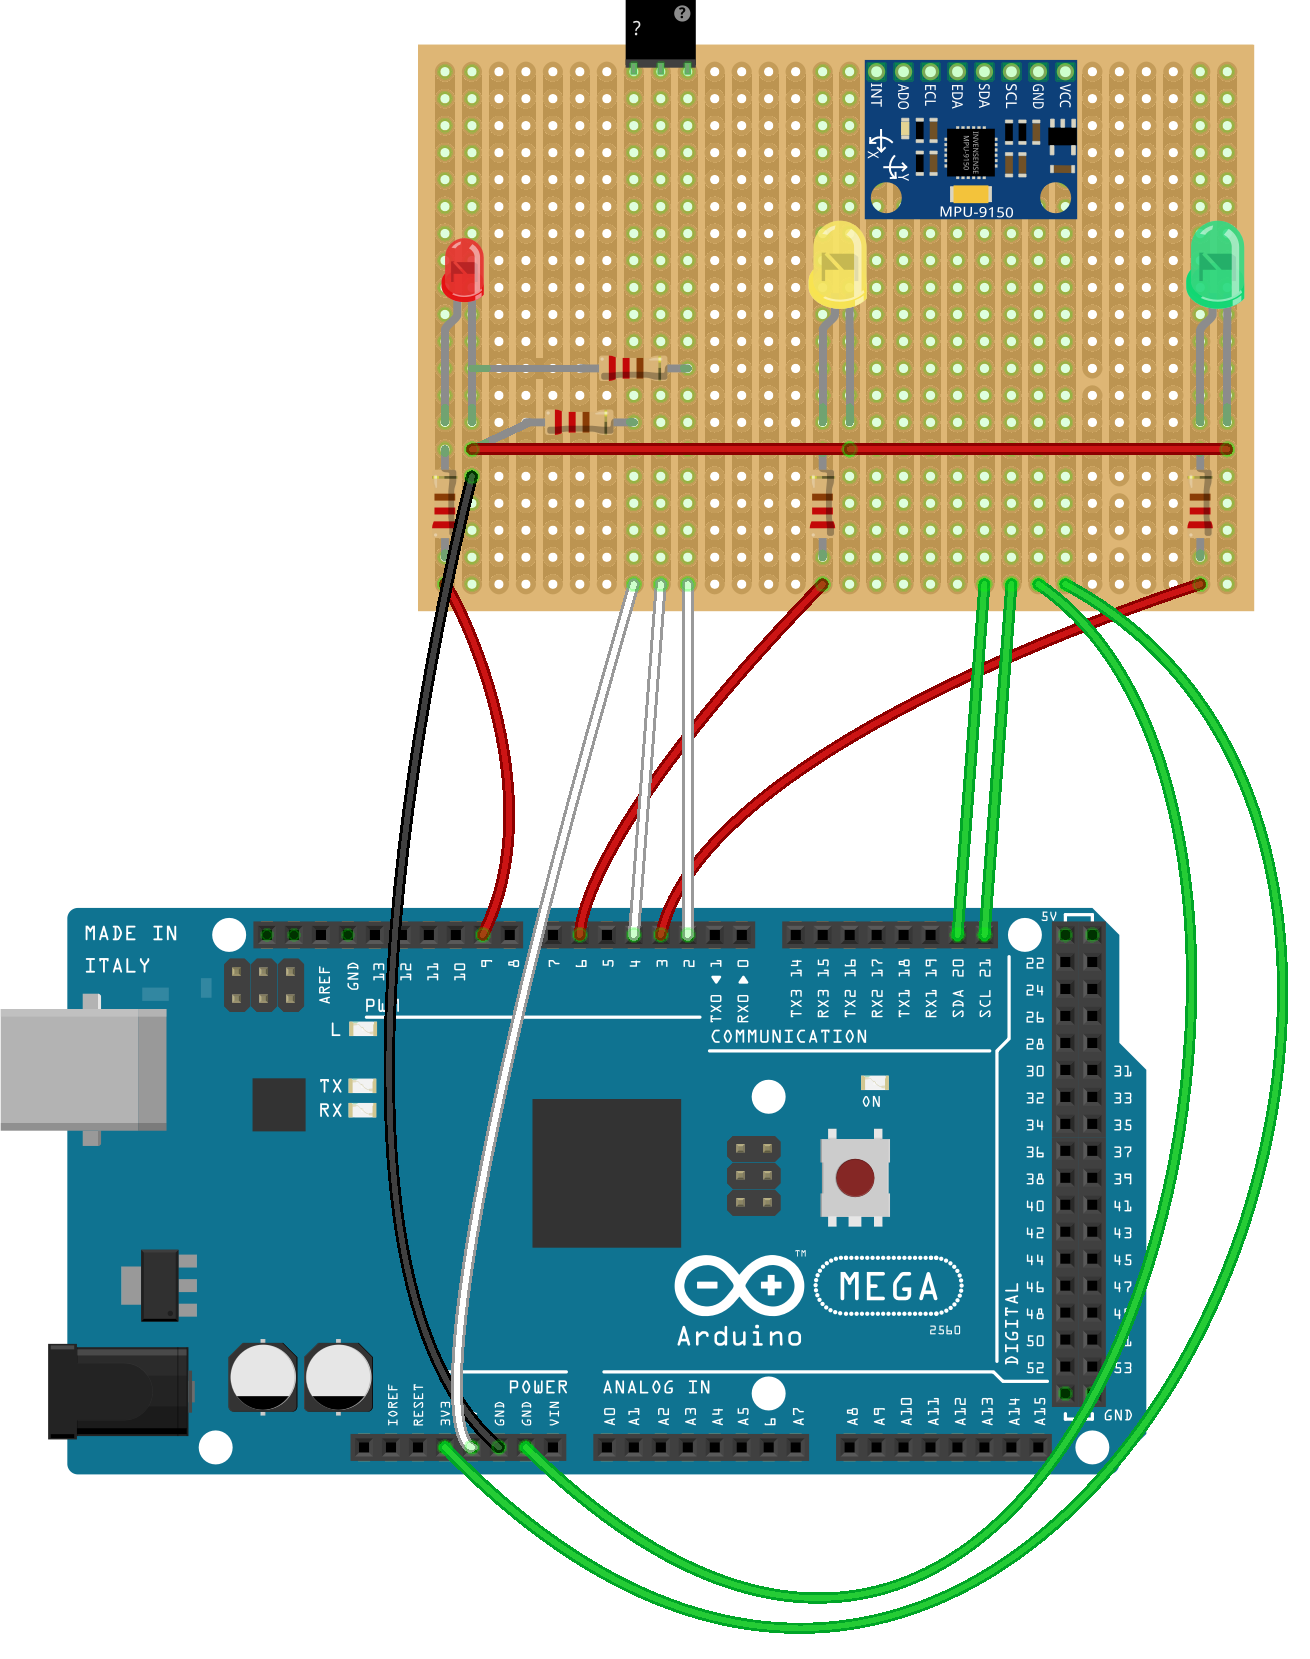
\includegraphics[keepaspectratio=true,scale=0.5]{Imu_Glove_Schematic}}
\captionof{figure}{Illustration of the prototype's circuit board }\label{schematic}
\end{minipage}\\

The circuit board consists of three LEDs - a red, a yellow and a green. They light up under different circumstances, which are explained in the next section of this chapter.

The LEDs are connected to resistors of 220 Ohm, which are wired to the Arduino as seen in figure \ref{schematic}. The green LED is connected to pin 3 on the Arduino. The yellow LED is connected to pin 6 and the red is connected to pin 9. This is essential to make it work in the Arduino code, which will be described later. 

The red wire connects all the LEDs and the black wire runs to the ground(GND) on the Arduino. The little blue circuit board on the yellow board represents the IMU. The necessary connections are: SDA, SCL, GND and VCC. 

SDA is the data line that sends data between the two devices, and the SCL is the clock line that sends pulses at a regular interval\citep{Arduino_SDA}. Every time the SCL changes from low to high, a single bit of information is sent over the SDA.

The SDA is connected to pin 20 and the SCL is connected to pin 21. GND is connected to ground on the Arduino and the VCC connection powers the sensor and is therefore connected to 3.3V pin on the Arduino. The white wires are also connected to the Arduino. The first wire from the left, which goes to the thumb, is connected to the 5V pin on the Arduino. The white wire beside it, is connected to the index finger, and pin 4 on the Arduino. The last white wire is connected to the middle finger and pin 2 on the Arduino. The wire which is connected to the thumb creates a circuit to the LEDs whenever the connection is created between either the thumb and index finger or thumb and middle finger. \\

The LEDs have to be connected to a pull-down resistor\citep{Pulldown_res}, which ensures that the Arduino does not 'float' between two different values. A pull-down resistor ensures, that the value is zero when no active device is connected.
Figure \ref{pull_down} shows a schematic with a pull-down resistor. \\


\begin{minipage}{\linewidth}% to keep image and caption on one page
\makebox[\linewidth]{%        to center the image
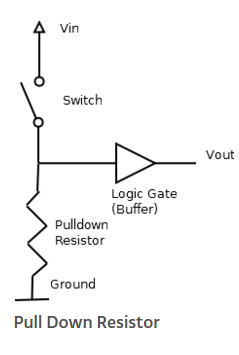
\includegraphics[keepaspectratio=true,scale=0.7]{Pull_down_resistor}}
\captionof{figure}{Schematic of pull-down resistor\citep{Pulldown_res}}\label{pull_down}
\end{minipage}\\

Figure \ref{prototype} shows the prototype. As one can see, the velcro for the fingers has copper tape on it, which has been glued onto the velcro. The velcro enables the user to wear the glove and to use it properly. 
 
This means that whenever the copper tape gets connected with the copper tape on the thumb, it creates the connection as mentioned earlier. 

The prototype has cloth sewed onto it, which makes it possible to wrap it around the wrist. \\

\begin{minipage}{\linewidth}% to keep image and caption on one page
\makebox[\linewidth]{%        to center the image
\includegraphics[keepaspectratio=true,scale=0.08]{FrontBack}}
\captionof{figure}{The front and back of the prototype}\label{prototype}
\end{minipage}

\subsection{Software}

This section describes the software part of the implementation. 

\subsubsection{Arduino}
The Arduino language is based on C/C++, and whenever a sketch is compiled, it is sent to a C/C++ compiler \citep{Arduino_FAQ}.\\

Information from the IMU is continually read and sent to the Arduino program. This data is then calculated by the Arduino program. It provides the pose, the angle, and the current movement of the IMU, all based on the data from the gyroscope, accelerometer and magnetometer.

The first part of the code shown in figure \ref{index_finger} reads the state of the copper plates. The following if-statement is executed whenever the index finger is connected with the thumb. 

If the user turns the hand to the left, the code sends the information to Pure Data, and if the hand is turned to the right, it sends that information. 

The direction of the hand determines the pitch within a value of 0-255. The motion is a rolling motion, which resembles the motion of turning a knob. \\


\begin{minipage}{\linewidth}% to keep image and caption on one page
\makebox[\linewidth]{%        to center the image
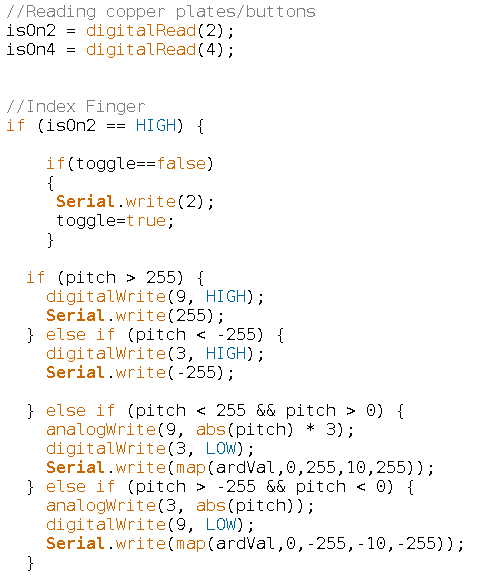
\includegraphics[keepaspectratio=true,scale=0.5]{Ardunio_Index_Finger}}
\captionof{figure}{Code describing what happens when the index finger is connected}\label{index_finger}
\end{minipage}\\

The code used for the middle finger is almost identical. It does however use different pins. Initially it was the plan to use the raise/lower movement for the pitch shifting, but since it caused some errors, it was decided to use the rolling motion for pitch also.\\

Figure \ref{Arduino_else} shows the last part of the code. This is an else statement that makes sure that the button is off whenever the copper plate is released. 

\begin{minipage}{\linewidth}% to keep image and caption on one page
\makebox[\linewidth]{%        to center the image
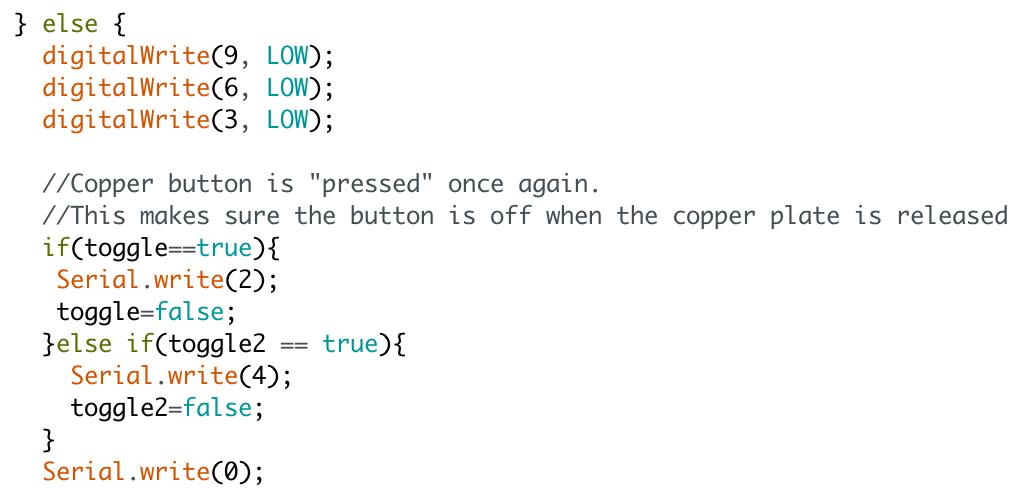
\includegraphics[keepaspectratio=true,scale=0.7]{Ardunio_else}}
\captionof{figure}{Else statement which makes sure the button is off when released}\label{Arduino_else}
\end{minipage}\\


\subsubsection{Pure Data}

The audio processing has been done in Pure Data(PD)\citep{PD_Info}, which is an open source programming language. It is used to generate and process sound, in a graphical way. 

The program uses patches where one can create objects which make it possible to create different audio effects. This subsection describes how PD has been used in this project, and explains the patches made for this project. \\

The first figure shows the main patch of the PD program, see figure \ref{PD_main}. The figure shows three coloured rectangles, red, green, and blue. 

The content of the red rectangle is Arduino related. PD gets data from the Arduino from the "comport" object, which is a serial port interface. 

The comport object needs a device number and a baud rate. In this case the device number is 1, and the baud rate is 4800 since this must be the same as the Arduino program's baud rate. The comport object takes three message objects as input: the name of the USB-device which starts the comport object, a message which shows which ports are available and a close message.   \\

\begin{minipage}{\linewidth}% to keep image and caption on one page
\makebox[\linewidth]{%        to center the image
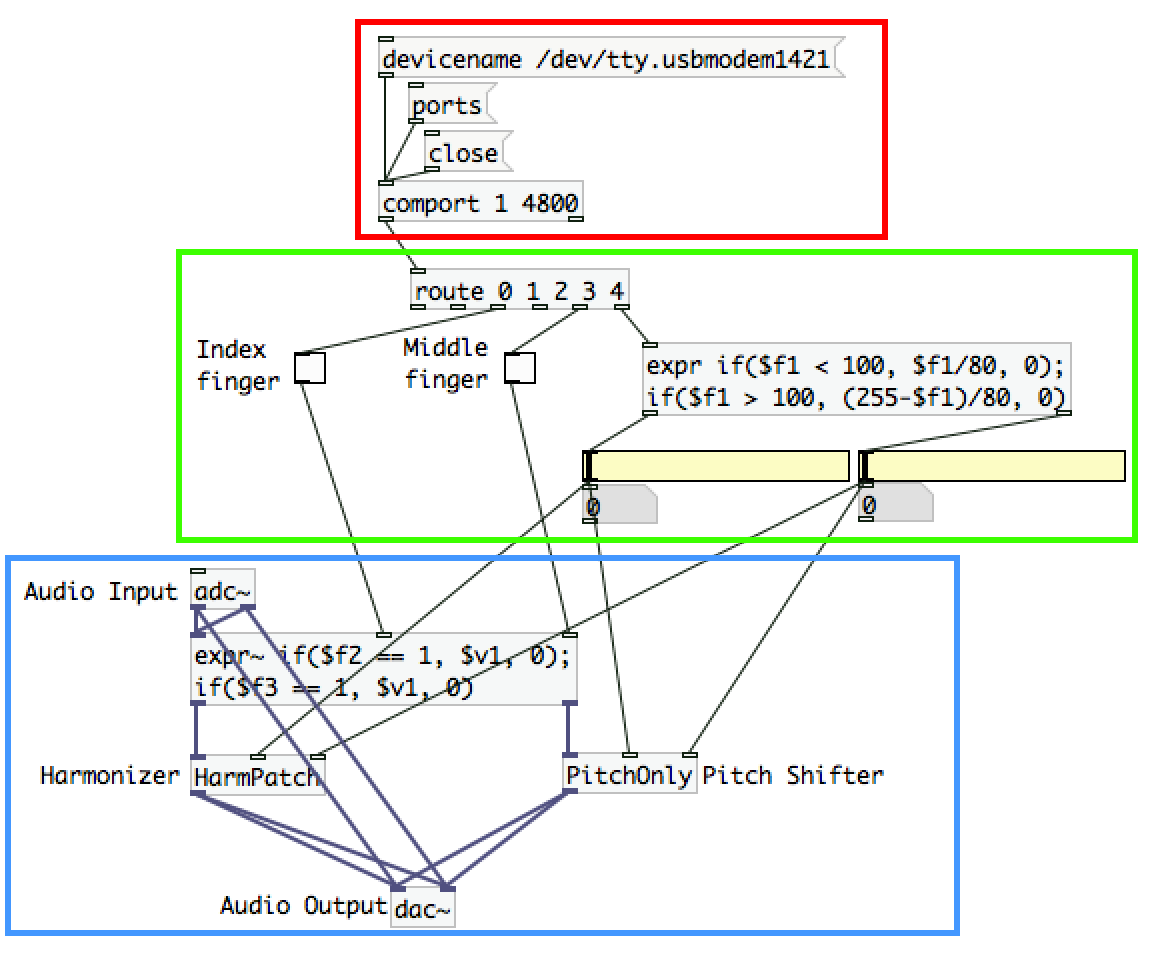
\includegraphics[keepaspectratio=true,scale=0.6]{PD_Main}}
\captionof{figure}{The main PD patch. Red rectangle is the Arduino part, green is the variable part, and blue is the effects part.}\label{PD_main}
\end{minipage}\\

The green rectangle processes the output from the comport object. The "route" object takes the data from the comport and splits it up into five parts. 

Route output number two and four correspond to the copper-plate buttons, e.g. if the index finger is connected, route output number two activates the toggle. 

The last route output is the sensor data, which goes to an "expr" object. The positive sensor data is between 10 and 100, and the negative between 255 and 155. 

The "expr" object splits the positive and negative values from each other, and divides them with 80. The negative values are subtracted from 255 first. The values go to two sliders.\\

The blue rectangle does the audio processing. Firstly, the "adc\textasciitilde" object which converts analog sound to digital takes the microphone input and sends into a "expr\textasciitilde" object. If the index finger is connected, 
the audio is sent to the "HarmPatch" patch, and if the middle finger is connected, the audio is sent to the "PitchOnly" patch. Both the "HarmPatch" and "PitchOnly" patches read the arguments of the sliders from the green rectangle. The outputs from the effects are then sent to the "dac\textasciitilde" object which converts digital sound to analog, which sends it to the sound output, in this case headphones.\\

Figure \ref{HarmPatch} illustrates the "HarmPatch" patch used for harmonising. As one can see in the figure, the audio coming from the "inlet\textasciitilde" object is sent to four "PitchShifter" objects. The "PitchShifter" object takes a message as an argument, which corresponds to the number of half tones one would like to pitch-shift. The two first "Pitchshifter" objects create a minor chord by pitch shifting by three and seven half tones.  The last two "PitchShifter" objects create a major chord by pitch shifting by four and seven half tones. The outputs from the four "PitchShifter" objects are then added in an "expr\textasciitilde" object, which uses the sensor input from the green rectangle from figure \ref{PD_main}. The output from the "expr\textasciitilde" object then goes to the "outlet" object.
 
\begin{minipage}{\linewidth}% to keep image and caption on one page
\makebox[\linewidth]{%        to center the image
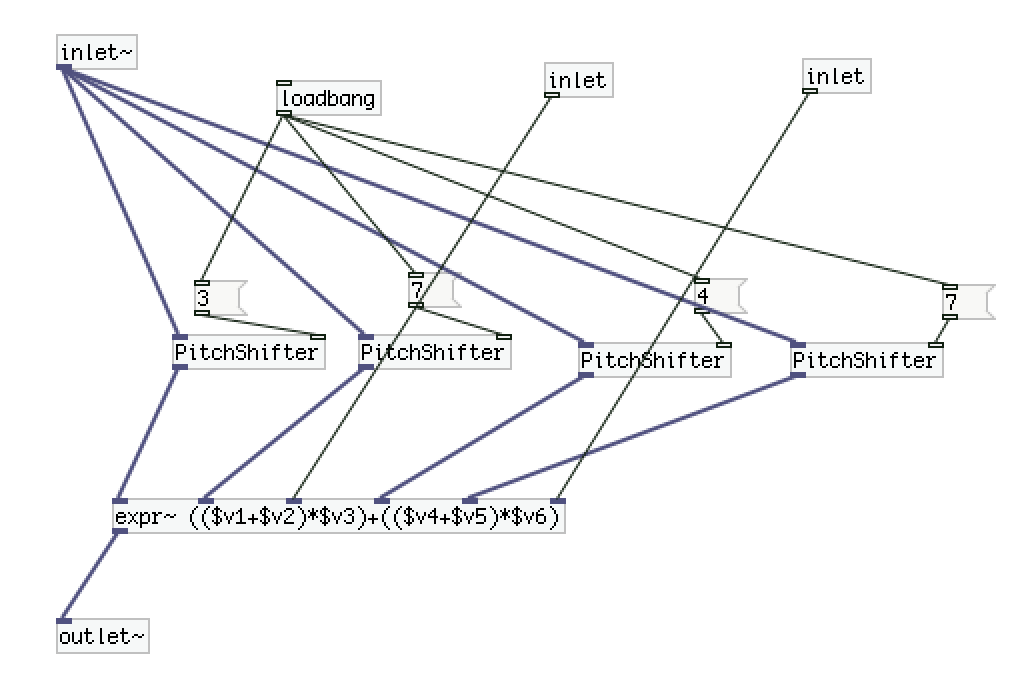
\includegraphics[keepaspectratio=true,scale=0.6]{HarmPatch}}
\captionof{figure}{The "HarmPatch" patch. The audio goes to four PitchShift patches, and are added together again after}\label{HarmPatch}
\end{minipage}\\

See figure \ref{Pitch_harm} for the Pitchshifting patch used in the harmoniser effect. The green rectangle receives a message, the half tone number, but must first convert it to a value that PD will use later. The conversion uses this equation (REF):

\[ 2^{h/12} = e^{0.05776*h} \] where h is the half tone number. E.g. three half tones would give the converted number 1.189. \\

\begin{minipage}{\linewidth}% to keep image and caption on one page
\makebox[\linewidth]{%        to center the image
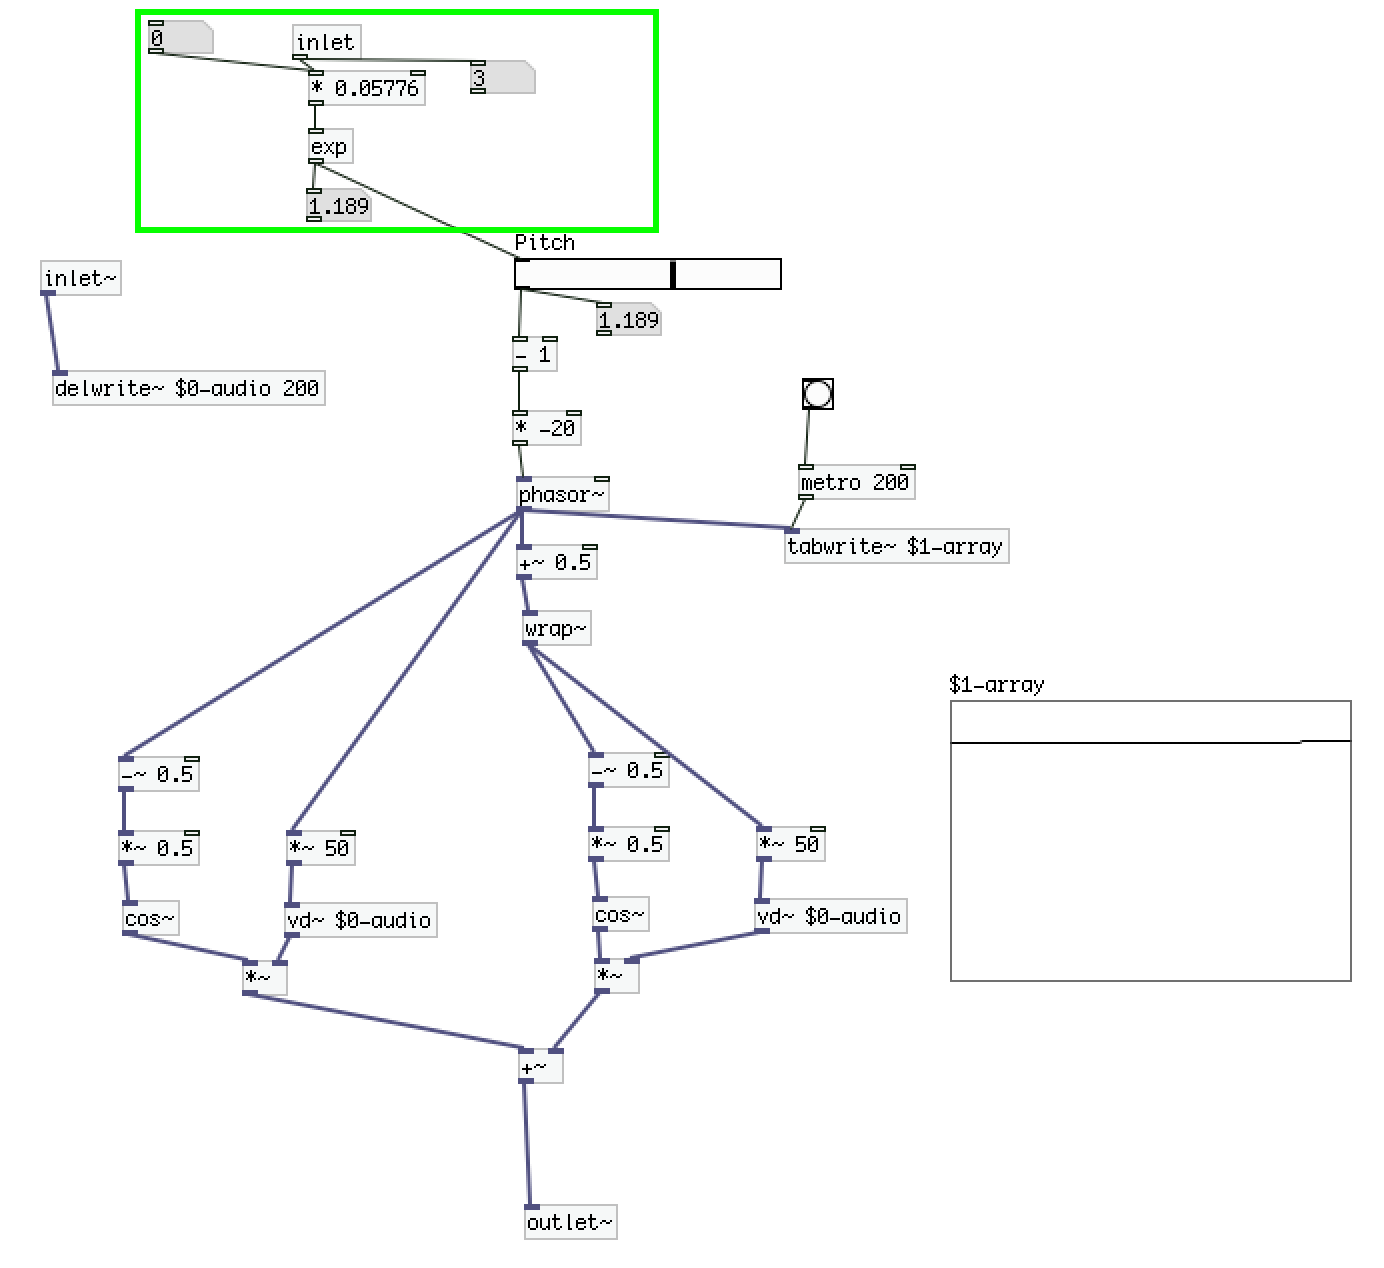
\includegraphics[keepaspectratio=true,scale=0.7]{Pitch_harm}}
\captionof{figure}{The Pitchshifting Patch used for the harmonize effect. The green rectangle is a bit different compared to the Pitchshifting effect.}\label{Pitch_harm}
\end{minipage}\\

The pitch shifting effect's patch does not convert numbers, but instead gets the slider data from the main patch, see the red box on figure \ref{Pitch_pitch}. Since the pitch shifting effect takes the input from 0-2, where 1 is regular pitch, the slider data is either added or subtracted with 1. 

\begin{minipage}{\linewidth}% to keep image and caption on one page
\makebox[\linewidth]{%        to center the image
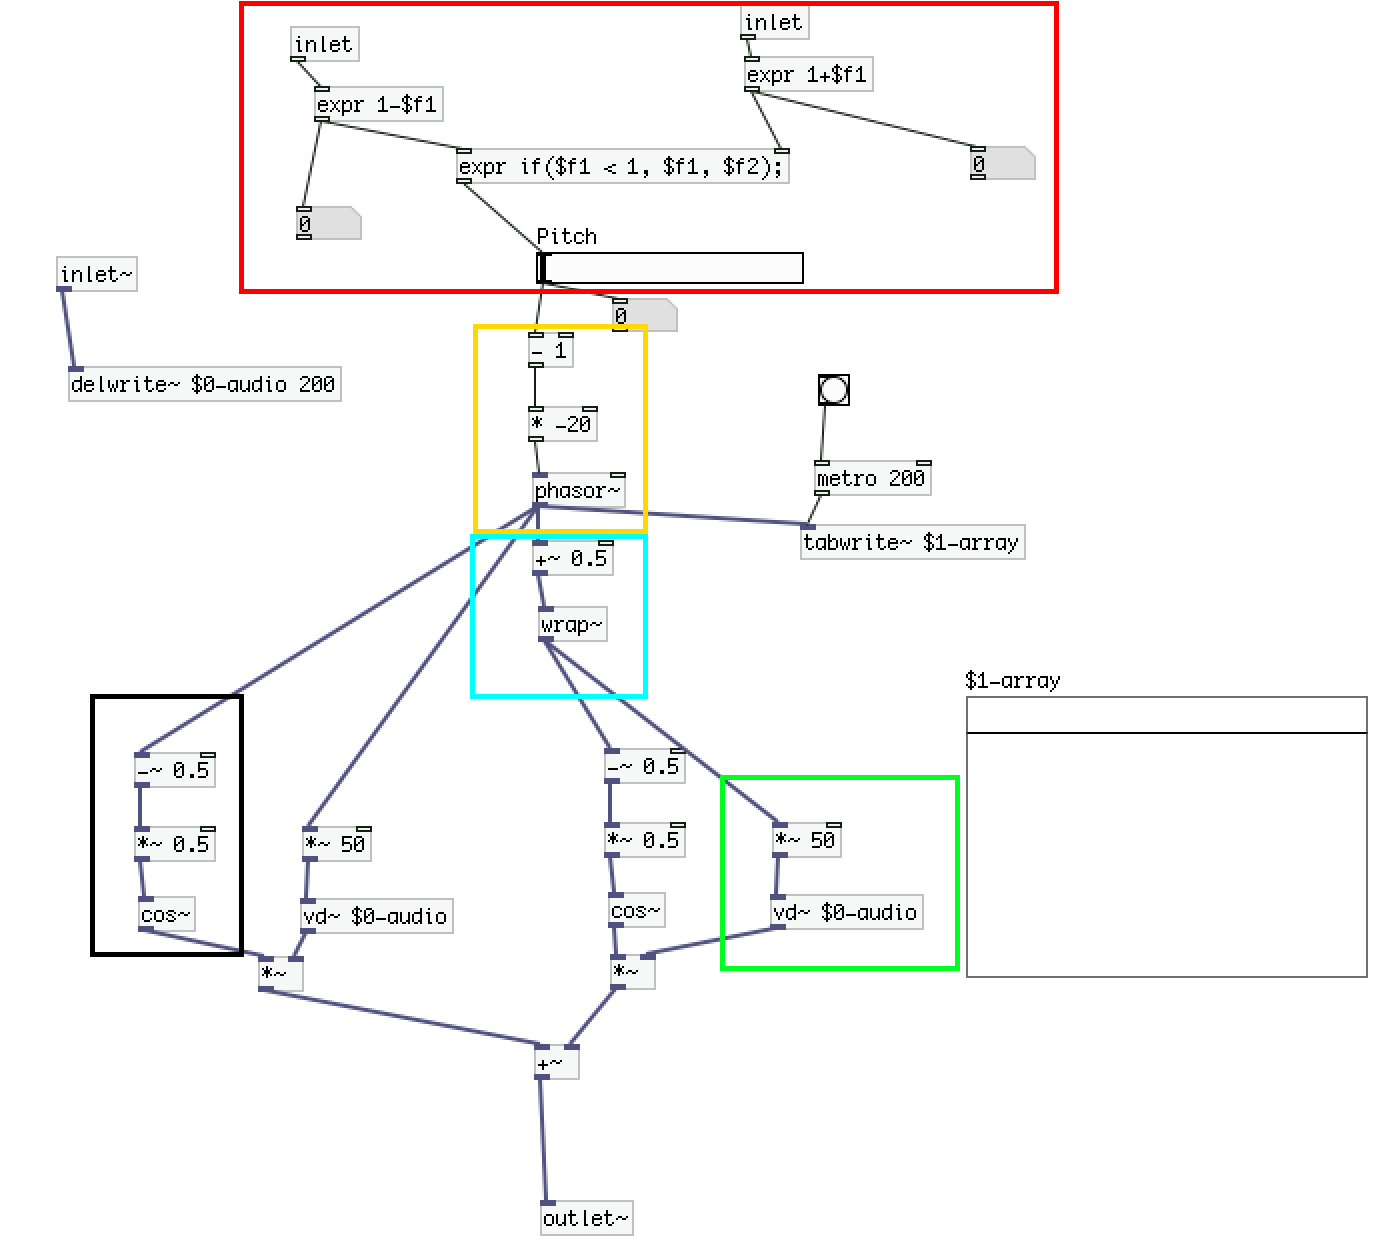
\includegraphics[keepaspectratio=true,scale=0.7]{PitchPatch}}
\captionof{figure}{The pitch shifting patch}\label{Pitch_pitch}
\end{minipage}\\

We find the delay by going through some steps. First, we find the difference between the "tape speed" and the original tape. Second, we multiply this number by -20. This is found by dividing the sample rate, 44100 Hz by the offset maximum, in this case 2205 samples, see the yellow square in figure \ref{Pitch_pitch}. The "phasor" object, which makes a sawtooth, takes the number we have just found as an input, and sends the output to the two delays. 

A phasor generates a sawtooth, and compared to the sinusoid, which goes from -1 to 1, the sawtooth goes from 0 to 1\citep{FlossManuals}. Normally, the sawtooth goes from low to high, and then abruptly to low again, as seen in figure \ref{sawtoothPic}. Since our tape head speed is going faster than the tape, it will progressively go to zero. In order to make the phasor fit with the delay, it must be inverted by making the input negative. It will go from high to low, and then to high again. This is why the 20 is negative in the yellow box.   

\begin{minipage}{\linewidth}% to keep image and caption on one page
\makebox[\linewidth]{%        to center the image
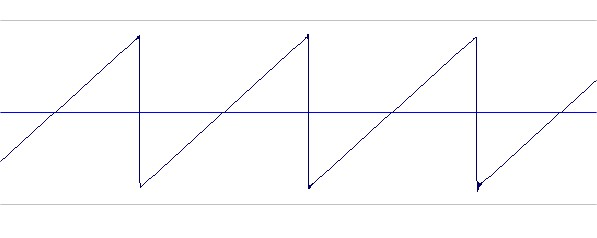
\includegraphics[keepaspectratio=true,scale=0.5]{sawtoothwave}}
\captionof{figure}{A Sawtooth wave\citep{Sawtooth}}\label{sawtoothPic}
\end{minipage}\\

The output of the phasor goes three ways. It goes to two variable delays, "vd\textasciitilde" objects, and two "cos" object. Before going to the "vd\textasciitilde" and "cos\textasciitilde" object on the right side of figure\ref{Pitch_pitch}, one output is shifted half a cycle by adding 0.5. In order to shift it back between zero and one, a "wrap" object is used which forces it between one and zero as seen in the blue box in figure \ref{Pitch_pitch}.\\

As mentioned before, the "vd\textasciitilde" objects are variable delays which get a varying delay time from the phasor. But before doing so the delay time is multiplied by 50, see the green box in figure\ref{Pitch_pitch}. This means that the "vd\textasciitilde" objects get a maximum delay time of 50 ms and a minimum of zero. A slight issue arises when the variable delay suddenly jumps because of the sawtooth wave and produces a click sound. In order to remove the clicking noise a smooth crossfade is used, which is done by using the "cos\textasciitilde" objects. Since the "vd\textasciitilde" and "cos\textasciitilde" objects on the right side of the figure\ref{Pitch_pitch} are half a cycle ahead of the left side, when one variable delay is in the maximum or minimum delay, the other is in the middle. Furthermore, using the "cos\textasciitilde" function the extreme high or low delays are faded out and this is called cosine windowing, see the black box in the figure\ref{Pitch_pitch}. The "cos\textasciitilde" objects on both sides are then multiplied by its "vd\textasciitilde" objects" and the results are then added and sent to the outlet. This leaves us with a pitch shifted output that has no clicks.  